% Theorie: Physikalische Grundlagen von Versuch/Messverfahren, Gleichungen ohne Herleitung knapp erklären
\section{Theorie}
\label{sec:theorie}

Ein Atom wird als stabil bezeichnet, wenn ein stabiles festgelegtes Verhältnis zwischen Neutronen und Protonen besteht.
Außerhalb dieser engen Grenze wandelt sich der Kern in einen stabilen oder instabilen Kern um.
Um die Zerfallswahrscheinlichkeit zu beschreiben wird die Halbwertszeit $T$ eines Nuklids bestimmt. Diese gibt bei einer 
großen Anzahl instabiler Kerne an, wann die Hälfte dieser zerfallen ist. Wenn die gesamte Nuklidkarte betrachtet wird, fällt auf, dass 
die verschiedenen Halbewertszeiten $T$ über 23 Zehnerpotenzen variieren können.
Im folgenden Experiment werden Halbwertszeiten bestimmt. Um Nuklide mit Halbwertszeiten im Sekunden bis Stunden Bereich herzustellen,
werden stabile Kernen mit Neutronen beschossen.

\subsection{Kernreaktionen mit Neutronen}
\label{sec:Kernreaktionen mit Neutronen}

Der Begriff Kernreaktion beschreibt allgemein die Wechselwirkungen von Teilchen mit Atomkernen.
Um die Halbwertszeiten bestimmen zu können, müssen zunächst Kernreaktionen, bei denen ein Neutron in ein Teilchen
eindringt, untersucht werden. Wird ein Atomkern mit einem Neutron beschossen, so wird der Kern in einen angeregten Zustand überführt.
Diese Kerne werden als Zwischenkern oder Compoundkern bezeichnet.
Die Energie des Compoundkerns ist um die kinetische Energie und die Bindungsenergie des Neutrons höher als
vorher. Durch die zusätzliche Enrgie entsteht die Anregung der Nukleonen. Der Kern ist in den meisten Fällen, wegen der
Verteilung der zusätzlichen Energie auf viele Nukleonen, nicht in der Lage, das Neutron oder ein Nukleon abzustoßen.
In diesem Falle wird ein $\gamma$-Quant emitiert, sodass der Zwischenkern wieder in den Grundzustand übergeht.
Für diese Reaktion gilt
\begin{equation}
    { }_z^m A+{ }_0^1 n \rightarrow{ }_z^{m+1} A^* \rightarrow{ }_z^{m+1} A+\gamma .
    \label{eqn:vorher}
\end{equation}
Der nun vorhandene Kern ist nicht stabil aufgrund der erhöhten Neutronenanzahl. Aufgrund des abgegebenen
Photons ist dieser langlebiger als der Compoundkern. Durch die Emission eines Elektrons geht dieser schließlich zu einem 
stabilen Kern über
\begin{equation}
    { }_z^{m+1} A \rightarrow \underset{z+1}{m+1} C+\beta^{-}+E_{k i n}+\bar{v}_e .
    \label{eqn:stabil}
\end{equation}
Die Masse von ${ }_z^{m+1} A$ ist größer als die Masse der Summe der Teilchen auf der rechten Seite der obigen Gleichung.
Gemäß der Einsteinschen Beziehung 
\begin{equation*}
    \Delta E = \Delta m c^2
\end{equation*}
wird die überschüssige Masse in kinetische Energie von Elektronen und Antineutrino umgewandelt.
Der Wirkungsquerschnitt $\sigma$ beschreibt die Wahrscheinlichkeit, dass ein Neutron durch einen stabilen Kern
eingefangen wird. Die durch den Wirkungsquerschnitt $\sigma$ beschreibt die Fläche, die der Kern haben sollte,
sodass jedes Neutron, welches diese Fläche trifft eingefangen wird. Für den Wirkungsquerschnitt gilt
\begin{equation}
    \sigma = \frac{u}{nKd}.
    \label{eqn:wirkungs}
\end{equation}
Dabei ist $d$ die Dicke der gegebenen Probe, n die Anzahl der auftreffenden Neutronen, $K$ die Anzahl der Kerne pro $\si{cm}^3$
und $u$ ist die Anzahl der eingefangen Neutronen.
Es liegt eine starke Abhängigkeit des Wirkungsquerschnittes von der Geschwindigkeit der Neutronen und damit von der
kinetischen Energie der Neutronen vor. Dementsprechend wird zwischen schnellen und langsamen Neutronen differenziert.
Anhand der De-Broglie-Wellenlänge $\lambda = \frac{h}{m_n v}$ kann ein Rückschluss gezogen werden.
Wenn die Geschwindigkeit $v$ der Neutronen sehr groß ist, sodass $\lambda$ klein gegen den Radius $R$ des gegebenen Kerns ist, dann
können für die Wechselwirkung der Neutronen mit dem Kern einfache geometrische Überlegungen verwendet werden.
Für die langsamen Neutronen bei denen gilt $R \leq \lambda$, können die geometrischen Überlegungen nicht angewendet werden.
Es lässt sich der Wirkungsquerschnitt als Funktion der Neutronenenergie $E$ darstellen. Die Formel von Breit und Wigner ist gegeben durch
\begin{equation}
    \sigma(E)=\sigma_0 \sqrt{\frac{E_{r_i}}{E}} \frac{\tilde{c}}{\left(E-E_{r_i}\right)^2+\tilde{c}} ,
    \label{eqn:funktion}
\end{equation}
wobei $\sigma_0$ und $\tilde{c}$ charakteristische Konstanten der betreffenden Kernreaktion sind und $E_{r_i}$
die Energieniveaus des Zwischenkerns darstellt.
In dem Fall, dass $ E \ll E_{r_i}$ gilt, kann der Term $\left(E-E_{r_i}\right)$ als konstant angenommen werden und
es folgt die Proportionalität
\begin{equation*}
    \sigma \sim \frac{1}{\sqrt{E}} \sim \frac{1}{v}.
\end{equation*}
Für den Versuch werden die niederenergetischen Neutronen benötigt, da die Wahrscheinlichkeit, dass diese eingefangen werden größer ist.

\subsection{Erzeugung niederenergetischen Neutronen}
\label{sec:Erzeugung niederenergetischen Neutronen}

Die gewollten niederenergetischen Neutronen müssen zunächst erzeugt werden. Neutronen kommen in der 
Natur als freies Teilchen nicht vor, da diese instabil sind. Daher muss es durch eine geeignete Kernreaktion 
hervor gebracht werden.
In dem Versuch werden die Neutronen durch Beschuss von $\ce{^{9}Be}$ mit $\alpha$-Teilchen freigesetzt
\begin{equation*}
    { }_4^9 \mathrm{Be}+{ }_2^4 \alpha \rightarrow{ }_6^{12} \mathrm{C}+{ }_0^1 \mathrm{n},
\end{equation*}
wobei die $\alpha$-Teilchen aus dem Zerfall $\ce{^{226}Ra}$ stammen. Zur Abbremsung werden
die Neutronen durch dicke Materieschichten hindurchdiffundiert.
Dabei kommt es zu elastischen Stößen mit den leichten Kernen der Atome und die Neutronen geben Energie ab.
Als Stoßpartner bietet sich das Wasserstoffatom an, da der Bremseffekt optimiert werden kann, indem die beiden sich stoßenden
Massen wenig verschieden sind. Die Neutronen werden soweit gebremst, dass die Energie ungefähr mit der mittleren kinetischen
Energie der Moleküle der Umgebung übereinstimmt. Diese Neutronen sind unter dem Begriff thermische Neutronen bekannt.

\subsection{Untersuchung des Zerfalls instabiler Isotope}
\label{sec:Untersuchung des Zerfalls instabiler Isotope}

Die Zahl $N(t)$ der zu dem Zeitpunkt $t$ noch nicht zerfallenen Kerne ist gegeben durch
\begin{equation}
    N(t) = N_0 e^{-\lambda t}.
    \label{eqn:zerfall}
\end{equation}
Hierbei sind $N_0$, die bei $t =0$ vorhandenen instabilen Kerne und $\lambda$ ist die Zerfallskonstante.
Die Zerfallskonstante beschreibt die Wahrscheinlichkeit  über die vorliegenden Zerfälle.
Die Halbwertszeit $T$ steht in Abhängigkeit zu $\lambda$ und es gilt
\begin{equation}
    T = \frac{\ln 2}{\lambda}.
    \label{eqn:Halbwertszeit}
\end{equation}
Gemessen wird für ein festes Zeitintervall $\Delta t$  die Anzahl der zerfallenen Kerne $N_{\Delta t}(t)$.
Dabei gilt die Gleichung 
\begin{equation*}
    N_{\Delta t}(t)=N(t)-N(t+\Delta t).
\end{equation*}
Durch das Einsetzten von \eqref{eqn:zerfall} folgt die Gleichung
\begin{equation}
    \ln N_{\Delta t}(t)=\ln N_0\left(1-e^{-\lambda \Delta t}\right)-\lambda t .
    \label{eqn:ausgleich}
\end{equation}
Mithilfe einer linearen Ausgleichsrechung lässt sich die Zerfallskonstante $\lambda$ bestimmen.

\subsection{Sonderfälle Rhodium und Silber}
\label{sec:Sonderfälle Rhodium und Silber}

Das natürlich vorkommende Silber besteht aus $52.3 \%$ aus dem Isotop $\ce{^{107}Ag}$ und zu $48.7 \%$
aus $\ce{^{109}Ag}$. Wird dieses mit Hilfe von Neutronen aktiviert, finden die Zerfälle zufällig statt.
Diese nebeneinander ablaufenden Zerfälle sind in \autoref{fig:neutron} dargestellt.

\begin{figure}[H]
    \centering
    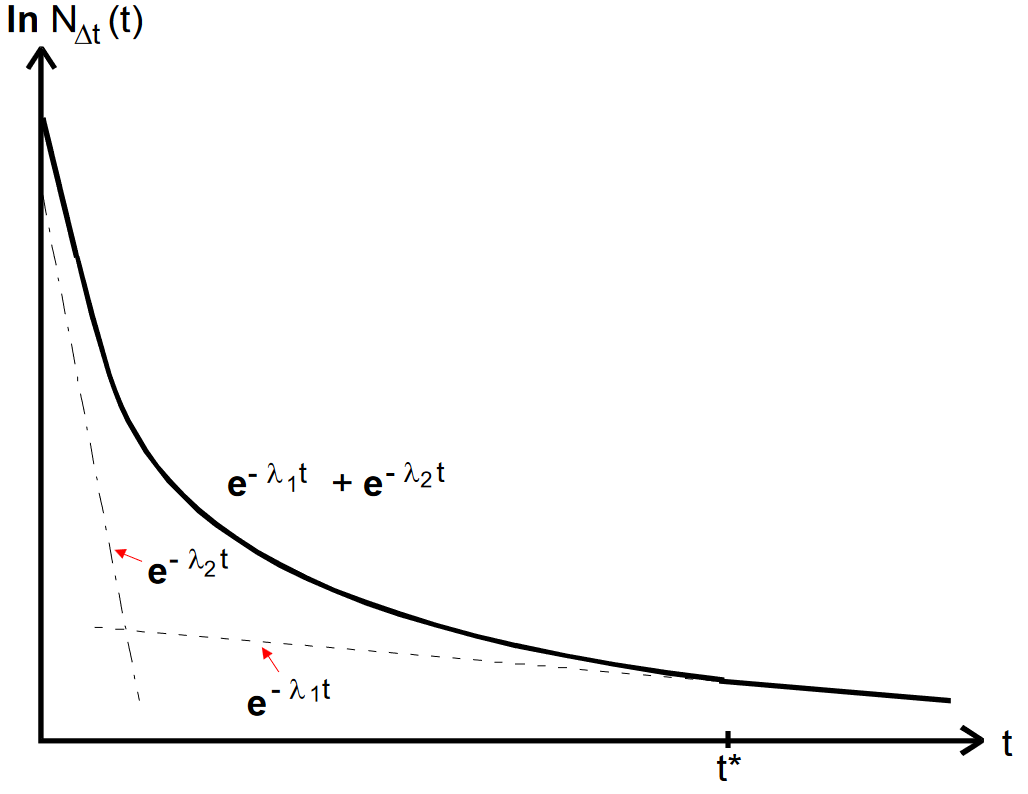
\includegraphics[width=0.8\linewidth]{content/grafik/zerfallskurve.png}
    \caption{Zerfalsskurve der Isotope von Silber.\cite{neutron}}
    \label{fig:neutron}
\end{figure}

Die Gesamtaktivität der Probe ist dabei die Summe der Einzelaktivitäten. Die Halbwertszeiten von
$\ce{^{107}Ag}$ und $\ce{^{109}Ag}$ weichen stark voneinander ab, was es möglich macht die jeweiligen
Halbwertszeiten zu bestimmen. Anhand der \autoref{fig:neutron} kann abgelesen werden, dass ab einem Zeitpunkt $t^*$
ausschließlich ein linearer Teil des Isotops mit längerer Hablwertszeit Einfluss hat. Mittels einer linearen Ausgleichsfunktion
lässt sich der Paramter $\lambda_l$ bestimmen. Über die Gleichung 
\begin{equation}
    \mathrm{N}_{\Delta \mathrm{t}_{\ell}}(\mathrm{t}):=\mathrm{N}_{0_{\ell}}\left(1-\mathbf{e}^{-\lambda_{\ell} \Delta \mathrm{t}}\right) \mathbf{e}^{-\lambda_{\ell} \mathrm{t}}
\end{equation}
kann die Zählrate berechnet werden. Die Zählrate der kurzlebigen Isotope ergibt sich aus der Differenz der gesamten gemessenen
Zählrate und der berechneten Werte der langlebigen Isotpe.

Das natürliche Rhodium besteht $100\%$ aus dem Isotop $\ce{^{103}Rh}$. Wird dieses aktiviert, so ensteht mit einer Wahrscheinlichkeit
von $90 \%$ das instabile Isotop $\ce{^{104}Rh}$. Andernfalls entseht aber auch das instabile $\ce{^{104i}Rh}$, welches 
durch die Emission eines $\gamma$-Quants in $\ce{^{104}Rh}$ übergeht. Beide Zerfälle laufen nebeneinander ab und das mit 
jeweils unterschiedlichen Halbwertszeiten. Es kann die gleiche Auswertungsmethode verwendet werden wie oben genannt, um
die Halbwertszeiten zu bestimmen.
